\documentclass[aspectratio=169,11pt]{beamer}

\usetheme[numbering=fraction,progressbar=frametitle]{metropolis}
\usepackage[T1]{fontenc}
\usepackage[utf8]{inputenc}
\usepackage{amsmath,amssymb}
\usepackage{booktabs}
\usepackage{listings}
\usepackage{xcolor}
\usepackage{tikz}
\usepackage{hyperref}

\definecolor{reuBlue}{HTML}{1F4E79}
\definecolor{reuOrange}{HTML}{D95F02}
\definecolor{reuGray}{HTML}{444444}
\definecolor{codeBg}{HTML}{F7F7F7}

\setbeamercolor{frametitle}{bg=reuBlue,fg=white}
\setbeamercolor{progress bar}{fg=reuOrange,bg=gray!25}
\setbeamercolor{alerted text}{fg=reuOrange}
\setbeamercolor{block title}{bg=reuBlue!15,fg=black}
\setbeamercolor{block body}{bg=gray!8,fg=black}

\lstdefinestyle{Rstyle}{
  language=R,
  basicstyle=\ttfamily\scriptsize,
  backgroundcolor=\color{codeBg},
  keywordstyle=\color{reuBlue}\bfseries,
  commentstyle=\color{reuGray}\itshape,
  stringstyle=\color{reuOrange},
  showstringspaces=false,
  frame=single,
  rulecolor=\color{gray!30},
  breaklines=true,
  columns=fullflexible
}
\lstset{style=Rstyle}

\title{Time Series Bootcamp}
\subtitle{Why time order matters, and how to forecast}
\author{Monnie McGee}
\institute{REU Bootcamp}
\date{June 10, 2026}

\begin{document}

\maketitle

\begin{frame}[fragile]{Software and Reference}

\textbf{Install once}

\begin{verbatim}
install.packages("fpp3")
install.packages("broom")
\end{verbatim}

\bigskip

\textbf{Load for this workshop}

\begin{verbatim}
library(fpp3)
library(broom)
\end{verbatim}

\bigskip

\textbf{Primary Reference}

Hyndman, R.J. \& Athanasopoulos, G. (2021), \emph{Forecasting: Principles and Practice} (3rd ed.)
\url{https://otexts.com/fpp3/}

\end{frame}

\begin{frame}{Two-hour learning goals}
By the end of this session, you should be able to:
\begin{enumerate}
  \item Recognize when data are time series data.
  \item Define autocorrelation.
  \item Explain why ordinary regression can be misleading for autocorrelated data.
  \item Identify trend, seasonality, cycles, and noise in a time plot.
  \item Describe forecasting as a train/test prediction problem.
  \item Fit and compare a few simple forecasting models in R.
\end{enumerate}

\vspace{0.4cm}
Reference spirit: Hyndman and Athanasopoulos, \emph{Forecasting: Principles and Practice}, 3rd ed.
\end{frame}

\section{1. Why ordinary regression often fails}

\begin{frame}{Temperature Example}
Suppose we record temperature every day.

\vspace{0.3cm}
\begin{block}{Question:}
If you know today's temperature, do you know something about tomorrow's temperature?
\end{block}

\pause

\vspace{0.3cm}
This is \alert{autocorrelation}: correlation between observations from the same series at different times.
\end{frame}

\begin{frame}{Regression assumption being challenged}
Ordinary least squares is often introduced with independent errors:
\[
  y_i = \beta_0 + \beta_1 x_i + \varepsilon_i,
  \qquad \varepsilon_i \text{ independent.}
\]

For time series, observations arrive in order:
\[
  y_t, y_{t-1}, y_{t-2}, \ldots
\]

A common time-series feature is:
\[
  \operatorname{Corr}(y_t, y_{t-1}) \neq 0.
\]

\alert{The past carries information about the future.}
\end{frame}

\begin{frame}[fragile]{Simulation: autocorrelated data with no trend}

\begin{lstlisting}[xleftmargin=0cm]
set.seed(123)

n <- 200
y <- numeric(n)

for(t in 2:n){
  y[t] <- 0.8 * y[t-1] + rnorm(1)
}

time <- 1:n
plot(time, y, type = "l",
     xlab = "Time", ylab = "y")

fit_lm <- lm(y ~ time)
summary(fit_lm)
\end{lstlisting}

\begin{tikzpicture}[remember picture,overlay]
\node[anchor=north east]
at ([xshift=-2cm,yshift=-2cm]current page.north east)
{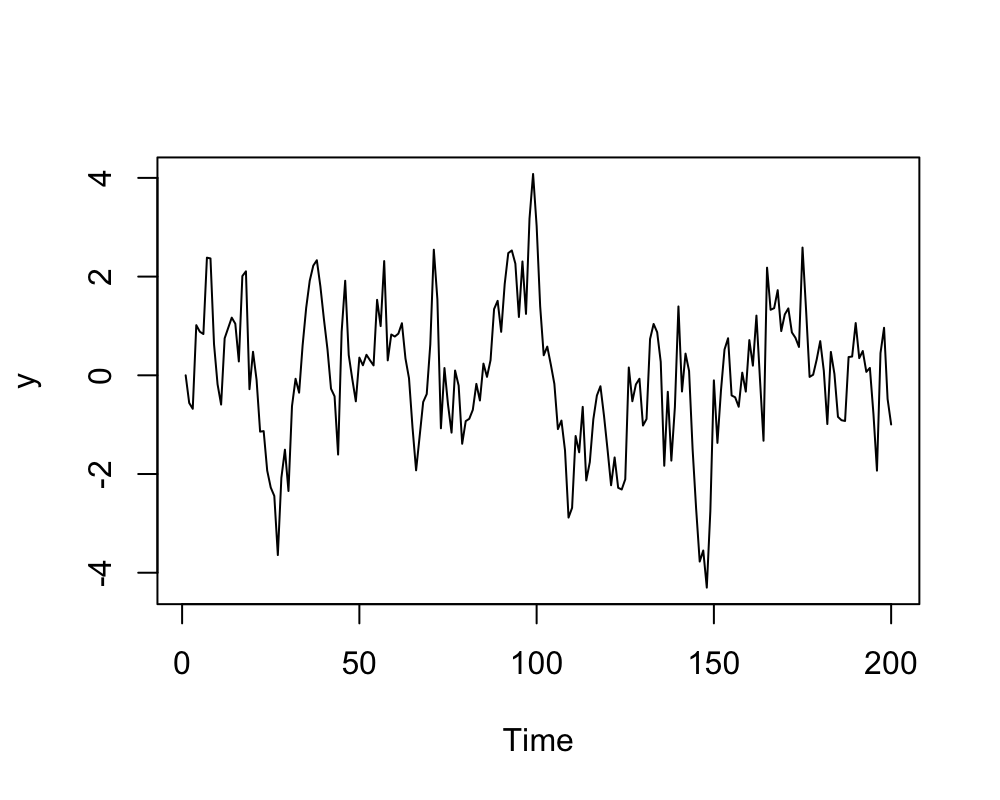
\includegraphics[width=7cm]{firstSeries.png}};
\end{tikzpicture}

The true process has no linear time trend, but it has long runs above and below zero.

\end{frame}

\begin{frame}[fragile]{Examine regression residuals}
\begin{lstlisting}
plot(residuals(fit_lm), type = "l",
     xlab = "Time", ylab = "Residual")
\end{lstlisting}

\pause
\vspace{0.4cm}
\begin{columns}
\column{0.4\textwidth}
Thought questions:
\begin{itemize}
  \item Do residuals look independent?
  \item Are there clusters of positive or negative residuals?
\end{itemize}

\column{0.6\textwidth}
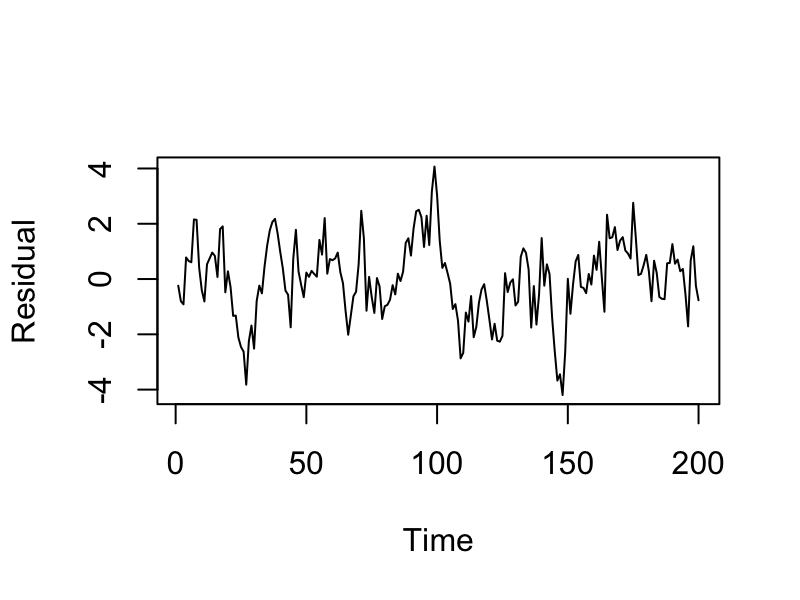
\includegraphics[width=7cm]{firstResids.png}
\end{columns}

\end{frame}

\begin{frame}{Important nuance: what exactly goes wrong?}
Autocorrelation alone does \alert{not} automatically make OLS slopes biased.

\vspace{0.2cm}
If the regression model is correctly specified and regressors are exogenous, OLS coefficients can still be unbiased.

\vspace{0.4cm}
But ordinary regression can still be badly misleading because:
\begin{itemize}
  \item standard errors and p-values can be wrong;
  \item trend or seasonality may be omitted;
  \item unrelated trending series can look strongly related;
  \item forecasts ignore useful information in recent observations.
\end{itemize}
\end{frame}

\begin{frame}{Strange Example: Temperature and CO$_2$}
Suppose we regress global temperature anomaly on atmospheric CO$_2$ concentration:
\[
  \text{Temperature}_t = \beta_0 + \beta_1\text{CO}_{2,t} + \varepsilon_t.
\]

Two of the most authoritative and stable public datasets for this topic:

NASA GISTEMP v4 is a data set of global mean temperature anomalies relative to the 1951–1980 baseline, updated monthly through the present. The file is a CSV pulled directly from \url{data.giss.nasa.gov}.

NOAA GML Mauna Loa annual mean $\text{CO}_2$ the longest continuous atmospheric $\text{CO}_2$ record, available as a CSV from \url{gml.noaa.gov.} 

Code to download and analyze data is in R Markdown File

\end{frame}

\begin{frame}{Climate Data Visuals}

\begin{center}
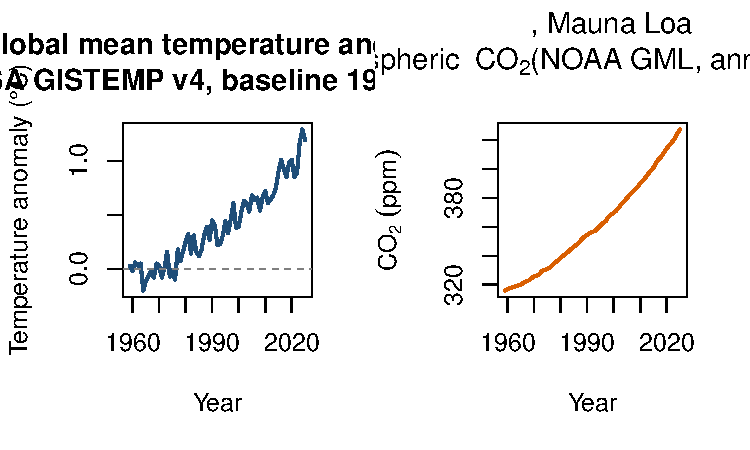
\includegraphics[scale=.7]{climatePlots.pdf}
\end{center}

The strong increase in $\text{CO}_2$ is very close to the trend in temperature. A linear regression will ``regress it out'', leaving almost white noise residuals.

\end{frame}

\begin{frame}{White Noise Residuals}

\begin{center}
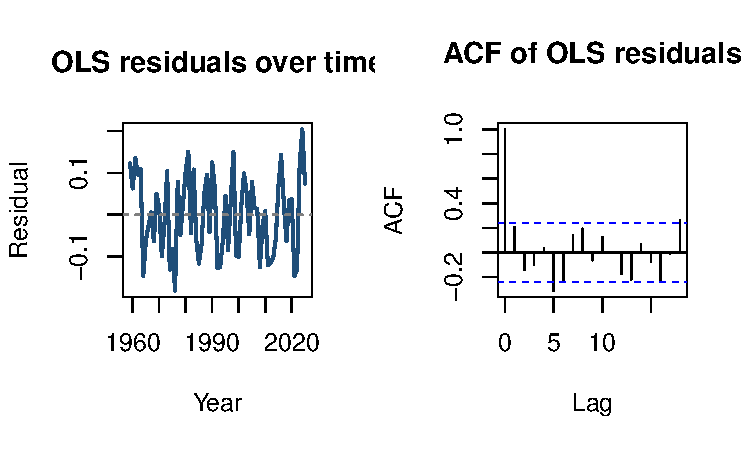
\includegraphics[scale=.7]{climateResids.pdf}
\end{center}

Because they share a common trend, but one series has a lot less noise than the other, a regression of temperature on $\text{CO}_2$ removes the trend, resulting in white noise residuals.

\end{frame}

\begin{frame}{Spurious regression}
Consider two independent random walks:
\[
  x_t = x_{t-1} + u_t,
  \qquad
  y_t = y_{t-1} + v_t.
\]

\vspace{0.2cm}
The error terms $u_t$ and $v_t$ are statistically independent, so the two series are unrelated.

\vspace{0.2cm}
But if both series wander over time, a regression of $y_t$ on $x_t$ may still produce:
\begin{itemize}
  \item a significant slope,
  \item a high $R^2$,
  \item autocorrelated residuals.
\end{itemize}
\end{frame}

\begin{frame}[fragile]{Your Turn: two independent random walks}
\begin{lstlisting}
set.seed(2026)

n <- 200
x <- cumsum(rnorm(n))
y <- cumsum(rnorm(n))
time <- 1:n

plot(time, x, type = "l", ylim = range(c(x, y)),
     xlab = "Time", ylab = "Value")
lines(time, y, lty = 2)
legend("topleft", legend = c("x", "y"), lty = c(1, 2), bty = "n")

fit_rw <- lm(y ~ x)
summary(fit_rw)
acf(residuals(fit_rw))
\end{lstlisting}

\vspace{0.2cm}
What do you see?
\end{frame}

\section{2. What makes time series different?}

\begin{frame}{Four common time-series features}
\begin{description}
  \item[Trend] Long-term movement upward or downward.
  \item[Seasonality] Repeating pattern with a fixed calendar period.
  \item[Cycles] Longer, less regular rises and falls.
  \item[Noise] Random variation left after structure is modeled.
\end{description}

\end{frame}

\begin{frame}{Other common examples}
\begin{tabular}{lll}
\toprule
Series & Likely structure & Forecasting use \\
\midrule
Daily temperature & seasonality, autocorrelation & weather planning \\
Monthly retail sales & trend, seasonality & inventory \\
Electricity demand & daily/weekly seasonality & grid management \\
Population & trend & planning services \\
Website traffic & trend, seasonality, shocks & staffing/content \\
\bottomrule
\end{tabular}

\vspace{0.5cm}
Time-series methods are appropriate when the order of observations carries information.
\end{frame}

\section{3. Forecasting mindset}

\begin{frame}{Regression mindset vs forecasting mindset}
\begin{columns}[T]
\column{0.48\textwidth}
\textbf{Regression mindset}
\begin{itemize}
  \item Estimate relationships.
  \item Interpret coefficients.
  \item Ask causal or explanatory questions.
\end{itemize}

\column{0.48\textwidth}
\textbf{Forecasting mindset}
\begin{itemize}
  \item Predict future observations.
  \item Evaluate accuracy on held-out data.
  \item A useful forecast need not be causal.
\end{itemize}
\end{columns}

\vspace{0.5cm}
In forecasting, the future is the test set.
\end{frame}

\begin{frame}{A basic forecasting task}
\begin{enumerate}
  \item Define what must be forecast.
  \item Decide the forecast horizon.
  \item Separate training data from future test data.
  \item Fit candidate models on training data.
  \item Compare forecasts to held-out observations.
\end{enumerate}

\vspace{0.4cm}
This is the workflow emphasized in forecasting texts such as FPP3.
\end{frame}

\begin{frame}[fragile]{Forecasting by Hand}
\begin{lstlisting}
library(fpp3)

recent_beer <- aus_production |>
  filter(year(Quarter) >= 1992)

train <- recent_beer |>
  filter(year(Quarter) <= 2007)

test <- recent_beer |>
  filter(year(Quarter) > 2007)

train |>
  autoplot(Beer) +
  autolayer(test, Beer, color = "gray") +
  labs(title = "Hide the future first")
\end{lstlisting}

\vspace{0.2cm}
Sketch the next few quarters before fitting any model.
\end{frame}

\section{Simple forecasting methods}

\begin{frame}{Three benchmark methods}
Before complicated models, use simple baselines.

\vspace{0.2cm}
\begin{description}
  \item[Mean forecast] Future values equal the historical average.
  \item[Naive forecast] Future values equal the most recent observation.
  \item[Seasonal naive] Future values equal the value from the same season last year.
\end{description}

\vspace{0.4cm}
A model is only impressive if it beats good baselines.
\end{frame}

\begin{frame}[fragile]{Fit benchmark forecasts in fpp3}
\begin{lstlisting}
fit_benchmarks <- train |>
  model(
    Mean = MEAN(Beer),
    Naive = NAIVE(Beer),
    Seasonal_naive = SNAIVE(Beer)
  )

fc_benchmarks <- fit_benchmarks |>
  forecast(h = nrow(test))

fc_benchmarks |>
  autoplot(train, level = NULL) +
  autolayer(test, Beer) +
  labs(title = "Benchmark forecasts")
\end{lstlisting}
\end{frame}

\begin{frame}[fragile]{Compare forecast accuracy}
\begin{lstlisting}
accuracy(fc_benchmarks, test)
\end{lstlisting}

\vspace{0.4cm}
Useful metrics:
\begin{itemize}
  \item RMSE: large errors are penalized heavily.
  \item MAE: average absolute error.
  \item MAPE: percentage error, but problematic near zero.
\end{itemize}

\vspace{0.3cm}
Keep the interpretation simple: lower error is better.
\end{frame}

\section{Exponential smoothing}

\begin{frame}{Forecasting tomorrow's temperature}
One simple forecast is the historical average:
\[
\hat y_{t+1} = \frac{y_1+y_2+\cdots+y_t}{t}.
\]

\vspace{0.4cm}
\begin{block}{Thought Question:}
Should a temperature from three years ago count as much as yesterday's temperature?
\end{block}

\vspace{0.3cm}
Makes sense to give more weight to recent observations.
\end{frame}

\begin{frame}{Exponentially weighted averages}
Exponential smoothing forecasts using weights that shrink as observations get older:
\[
\hat y_{t+1}
=
\alpha y_t
+\alpha(1-\alpha)y_{t-1}
+\alpha(1-\alpha)^2y_{t-2}
+\cdots.
\]

\vspace{0.4cm}
\begin{block}{Main idea}
Recent observations matter most, but older observations are not thrown away completely.
\end{block}
\end{frame}

\begin{frame}{The recursive form}
Simple exponential smoothing can be written as
\[
\ell_t = \alpha y_t + (1-\alpha)\ell_{t-1}.
\]

\vspace{0.3cm}
Here \(\ell_t\) is the current estimate of the level.

\vspace{0.4cm}
\begin{block}{Plain-language interpretation}
New estimate = weighted average of what we just observed and what we previously believed.
\end{block}
\end{frame}

\begin{frame}{What does \(\alpha\) do?}
\begin{center}
\begin{tabular}{lll}
\toprule
Value of \(\alpha\) & Behavior & Interpretation \\
\midrule
Small, such as 0.1 & Very smooth & Slow to adapt \\
Medium, such as 0.5 & Balanced & Moderate adaptation \\
Large, such as 0.9 & Wiggly & Responds quickly \\
\bottomrule
\end{tabular}
\end{center}

\vspace{0.4cm}
\begin{block}{Key intuition}
The smoothing parameter controls the tradeoff between stability and responsiveness.
\end{block}
\end{frame}

\begin{frame}[fragile]{Manual demonstration of \(\alpha\)}
\begin{lstlisting}
ses_level <- function(y, alpha) {
  level <- numeric(length(y))
  level[1] <- y[1]

  for (t in 2:length(y)) {
    level[t] <- alpha*y[t] + (1 - alpha)*level[t - 1]
  }

  level
}

beer <- aus_production |>
  filter_index("1990 Q1" ~ "2005 Q4") |>
  select(Quarter, Beer)
\end{lstlisting}
\end{frame}

\begin{frame}[fragile]{Plot three smoothers}
\begin{lstlisting}
beer_smooth <- beer |>
  mutate(
    alpha_10 = ses_level(Beer, 0.10),
    alpha_50 = ses_level(Beer, 0.50),
    alpha_90 = ses_level(Beer, 0.90)
  )

beer_smooth |>
  pivot_longer(alpha_10:alpha_90,
               names_to = "alpha", values_to = "smooth") |>
  ggplot(aes(x = Quarter)) +
  geom_line(aes(y = Beer), color = "gray60") +
  geom_line(aes(y = smooth, color = alpha)) +
  labs(y = "Beer production", color = "Smoother")
\end{lstlisting}
\end{frame}

\begin{frame}[fragile]{Fit exponential smoothing with fpp3}
\begin{lstlisting}
fit_ets <- beer |>
  model(ETS(Beer))

report(fit_ets)
\end{lstlisting}

\vspace{0.4cm}
\begin{block}{What R is doing}
\texttt{ETS()} chooses an exponential smoothing model for error, trend, and seasonality.
\end{block}
\end{frame}

\begin{frame}[fragile]{Forecast with exponential smoothing}
\begin{lstlisting}
fc_ets <- fit_ets |>
  forecast(h = "2 years")

fc_ets |>
  autoplot(beer) +
  labs(y = "Beer production",
       title = "Exponential smoothing forecast")
\end{lstlisting}

\end{frame}

\begin{frame}{Trend and seasonality extensions}
\begin{center}
\begin{tabular}{ll}
\toprule
Pattern in the data & Common method \\
\midrule
No trend, no seasonality & Simple exponential smoothing \\
Trend & Holt's method \\
Trend plus seasonality & Holt-Winters method \\
\bottomrule
\end{tabular}
\end{center}

\vspace{0.4cm}
\begin{block}{Keep the message simple}
Exponential smoothing is a family of forecasting methods, not just one formula.
\end{block}
\end{frame}

\section{ARIMA as the next thing to learn}

\begin{frame}{Autoregression: the next model idea}
An autoregressive model predicts future values using previous values:
\[
Y_t = \phi Y_{t-1} + \varepsilon_t.
\]

\vspace{0.4cm}
\begin{block}{Contrast}
Exponential smoothing predicts by smoothing the past. AR models predict by explicitly modeling dependence on previous observations.
\end{block}
\end{frame}

\begin{frame}{Where ARIMA enters}
ARIMA combines three ideas:
\begin{itemize}
  \item \textbf{AR}: autoregression, using past values
  \item \textbf{I}: differencing, removing trend or nonstationarity
  \item \textbf{MA}: moving average errors, using past shocks
\end{itemize}

\vspace{0.4cm}
\begin{block}{Bootcamp-level takeaway}
ARIMA is important, but it is a next step after understanding forecasting, autocorrelation, training/test data, and benchmark methods.
\end{block}
\end{frame}

\begin{frame}[fragile]{A minimal ARIMA example}
\begin{lstlisting}
fit_arima <- beer |>
  model(ARIMA(Beer))

report(fit_arima)

fit_arima |>
  forecast(h = "2 years") |>
  autoplot(beer)
\end{lstlisting}

\vspace{0.3cm}
The goal is not to explain every parameter. The goal is to show the workflow.
\end{frame}

\begin{frame}[fragile]{Simulate different levels of persistence}
\begin{lstlisting}
set.seed(1)

low_persistence  <- arima.sim(list(ar = 0.2), n = 200)
high_persistence <- arima.sim(list(ar = 0.8), n = 200)
near_random_walk  <- arima.sim(list(ar = 0.98), n = 200)

plot(low_persistence, type = "l", main = "phi = 0.2")
plot(high_persistence, type = "l", main = "phi = 0.8")
plot(near_random_walk, type = "l", main = "phi = 0.98")
\end{lstlisting}

\vspace{0.2cm}
Ask: Which series is easiest to forecast tomorrow? Which is hardest long-term?
\end{frame}

\begin{frame}[fragile]{Fit a simple ARIMA model}
\begin{lstlisting}
fit_arima <- train |>
  model(ARIMA(Beer))

report(fit_arima)

fc_arima <- fit_arima |>
  forecast(h = nrow(test))

fc_arima |>
  autoplot(train) +
  autolayer(test, Beer) +
  labs(title = "ARIMA forecast")
\end{lstlisting}

\vspace{0.2cm}
ARIMA models use autocorrelation and differencing to forecast.
\end{frame}

\begin{frame}{A gentle explanation of differencing}
If a series has a strong trend, model the changes instead of the levels:
\[
  \Delta Y_t = Y_t - Y_{t-1}.
\]

\vspace{0.3cm}
Differencing often turns a wandering nonstationary series into a more stable series.

\vspace{0.4cm}
This connects directly to the random-walk demo:
\[
  Y_t = Y_{t-1} + \varepsilon_t
  \quad \Rightarrow \quad
  \Delta Y_t = \varepsilon_t.
\]
\end{frame}

\section{Modern workflow checklist}

\begin{frame}{Time-series workflow checklist}
When you see data collected over time:

\begin{enumerate}
  \item Plot the series.
  \item Look for trend.
  \item Look for seasonality.
  \item Check autocorrelation.
  \item Split into training and test periods.
  \item Fit simple baselines.
  \item Fit time-series models and compare forecast accuracy.
\end{enumerate}
\end{frame}

\begin{frame}{When are time-series methods appropriate?}
Use time-series methods when:
\begin{itemize}
  \item observations are ordered in time;
  \item nearby observations tend to be related;
  \item trend or seasonality is part of the signal;
  \item the goal is forecasting future observations;
  \item residuals from ordinary regression are autocorrelated.
\end{itemize}

\vspace{0.4cm}
A time series is not just a dataset with a date column. The date order must matter.
\end{frame}

\begin{frame}{Take-home message}
\begin{center}
\Large
Regression treats observations as exchangeable rows.\\[0.4cm]
Time series treats observations as ordered history.\\[0.6cm]
\alert{The past is information.}
\end{center}
\end{frame}

\section{And now for something completely different}

\begin{frame}{Why include these?}
These methods are not time series methods, but they are useful in general data analysis situations.

\vspace{0.3cm}
\begin{enumerate}
  \item \textbf{Bootstrap}: quantify uncertainty by resampling data.
  \item \textbf{Local linear regression smoothing}: reveal nonlinear relationships.
  \item \textbf{Kernel density estimation}: estimate the shape of a distribution.
\end{enumerate}

\vspace{0.3cm}
Each one is a practical alternative to relying only on formulas from idealized models.
\end{frame}

\section{Bootstrap}

\begin{frame}{Bootstrap: the idea}
Suppose we have a sample \(x_1,\ldots,x_n\) and want uncertainty for a statistic.

\vspace{0.3cm}
\begin{block}{Bootstrap logic}
If the sample is our best guess of the population, repeatedly resample from the sample and recompute the statistic.
\end{block}

\vspace{0.3cm}
This gives an approximate sampling distribution.
\end{frame}

\begin{frame}[fragile]{Bootstrap a mean in R}
\begin{lstlisting}
set.seed(123)

x <- na.omit(airquality$Ozone)

boot_means <- replicate(2000, {
  x_star <- sample(x, size = length(x), replace = TRUE)
  mean(x_star)
})

quantile(boot_means, c(0.025, 0.975))
\end{lstlisting}

\vspace{0.3cm}
This is a bootstrap confidence interval for the mean ozone level.
\end{frame}

\begin{frame}[fragile]{Visualize the bootstrap distribution}
\begin{lstlisting}
tibble(boot_mean = boot_means) |>
  ggplot(aes(x = boot_mean)) +
  geom_histogram(bins = 30) +
  labs(x = "Bootstrap means",
       y = "Count",
       title = "Bootstrap sampling distribution")
\end{lstlisting}

\vspace{0.3cm}
The spread of this distribution represents uncertainty in the estimate.
\end{frame}

\section{Local linear regression smoothing}

\begin{frame}{Local smoothing: the idea}
Linear regression fits one global line.

\vspace{0.3cm}
Local regression fits many small regressions near each value of \(x\).

\vspace{0.4cm}
\begin{block}{Why it helps}
It reveals nonlinear patterns without forcing a single polynomial or a single straight line.
\end{block}
\end{frame}

\begin{frame}{Local linear regression in words}
To estimate the curve near a point \(x_0\):
\begin{enumerate}
  \item Give observations near \(x_0\) high weight.
  \item Give observations far from \(x_0\) low weight.
  \item Fit a small weighted regression locally.
  \item Move \(x_0\) across the plot to trace out a smooth curve.
\end{enumerate}

\vspace{0.3cm}
The bandwidth or span controls how smooth the curve is.
\end{frame}

\begin{frame}[fragile]{Local regression smoothing in R}
\begin{lstlisting}
ggplot(mtcars, aes(x = wt, y = mpg)) +
  geom_point() +
  geom_smooth(method = "loess", se = FALSE) +
  labs(x = "Weight",
       y = "Miles per gallon",
       title = "Local regression smoother")
\end{lstlisting}

\vspace{0.3cm}
Use this as an exploratory tool, not as automatic proof of a relationship.
\end{frame}

\section{Kernel density estimation}

\begin{frame}{Kernel density estimation: the idea}
A histogram estimates the shape of a distribution, but it depends heavily on bin width and bin edges.

\vspace{0.3cm}
Kernel density estimation places a small smooth bump at each observation and adds the bumps together.

\vspace{0.4cm}
\begin{block}{Main idea}
KDE is a smooth version of a histogram.
\end{block}
\end{frame}

\begin{frame}{Bandwidth matters}
\begin{center}
\begin{tabular}{ll}
\toprule
Bandwidth choice & Result \\
\midrule
Too small & Too wiggly \\
Reasonable & Reveals the distribution shape \\
Too large & Over-smoothed \\
\bottomrule
\end{tabular}
\end{center}

\vspace{0.4cm}
The bandwidth plays a role similar to \(\alpha\) in smoothing: it controls flexibility.
\end{frame}

\begin{frame}[fragile]{Kernel density estimation in R}
\begin{lstlisting}
ggplot(mtcars, aes(x = mpg)) +
  geom_histogram(aes(y = after_stat(density)), bins = 10) +
  geom_density(linewidth = 1) +
  labs(x = "Miles per gallon",
       y = "Density",
       title = "Histogram plus kernel density estimate")
\end{lstlisting}

\vspace{0.3cm}
We can see the distribution without choosing many arbitrary bins.
\end{frame}


\begin{frame}{Suggested activity}
Examine a data set from FPP3 and answer three questions:

\vspace{0.3cm}
\begin{enumerate}
  \item What patterns do you see in the plot?
  \item Which forecast would you trust for the next few observations?
  \item How would you quantify uncertainty or reveal structure if this were not a time series?
\end{enumerate}

\end{frame}


\end{document}
